\chapter{Thử nghiệm và kết quả}

\section{Các mô hình Baseline đối chứng}
Để đánh giá chính xác giá trị gia tăng của các kỹ thuật tinh chỉnh và tiền xử lý, nhóm thiết lập ba mốc đối chứng (baseline) theo đúng khuyến nghị của hướng dẫn học phần:
\begin{enumerate}
    \item \textbf{Baseline lớp đa số (Zero-R / Majority Class)}: Dự đoán mọi mẫu đều thuộc lớp \texttt{Graduate} (chiếm 49,9\% dữ liệu huấn luyện). Mốc này đạt Accuracy $0{,}4994$ trên tập kiểm thử nhưng Macro-F1 chỉ đạt $0{,}2221$, và hoàn toàn bất lực trong việc cảnh báo nguy cơ bỏ học (Recall Dropout bằng $0{,}0000$).
    \item \textbf{Baseline K-NN mặc định (Default K-NN)}: Sử dụng cấu hình tiêu chuẩn của scikit-learn ($k=5$, trọng số biểu quyết đều, khoảng cách Euclid $p=2$) kết hợp với Luồng A cơ bản (không tinh chỉnh siêu tham số). Trên 5-fold CV, mô hình đạt Macro-F1 $0{,}4401 \pm 0{,}0140$; trên tập test đạt Accuracy $0{,}4972$ và Macro-F1 $0{,}4126$.
    \item \textbf{Baseline Cây quyết định mặc định (Default Decision Tree)}: Cây phát triển tự do không giới hạn độ sâu (\texttt{max\_depth=None}), tiêu chí Gini, không trọng số lớp. Trên 5-fold CV mô hình đạt Macro-F1 $0{,}4241 \pm 0{,}0205$; trên tập test đạt Accuracy $0{,}4825$ và Macro-F1 $0{,}4347$.
\end{enumerate}

\section{Kết quả kiểm định chéo và lựa chọn siêu tham số}
Cả bốn tổ hợp thử nghiệm chính được huấn luyện trên 3.539 mẫu train với cùng bộ 5 fold phân tầng. Không gian siêu tham số được duyệt đầy đủ bằng \texttt{GridSearchCV} theo tiêu chí tối đa hóa Macro-F1 CV. Cấu hình được chọn và điểm số kiểm định chéo được trình bày trong Bảng~\ref{tab:cv}. Phép thử bổ sung giữ nguyên các tham số khác của B/cây cho macro-F1 CV 0,4508 với Gini và 0,4544 với entropy; đây là phép khảo sát trên train, không dùng để chọn lại bằng test.

\begin{table}[H]\centering\small
\caption{Cấu hình siêu tham số tối ưu chọn theo 5-fold CV trên tập train}\label{tab:cv}
\begin{tabular}{p{2.2cm}p{8.8cm}r}\toprule
Tổ hợp & Siêu tham số tối ưu được chọn & Macro-F1 CV\\\midrule
A / K-NN & $k=5$; khoảng cách Manhattan ($p=1$); trọng số đều (\texttt{uniform}) & 0,4455\\
A / Cây & \texttt{max\_depth=12}; \texttt{min\_samples\_leaf=10}; \texttt{class\_weight=None} & 0,4508\\
B / K-NN & $k=11$; khoảng cách Manhattan ($p=1$); trọng số đều (\texttt{uniform}) & 0,4661\\
B / Cây & \texttt{max\_depth=12}; \texttt{min\_samples\_leaf=1}; \texttt{class\_weight='balanced'} & 0,4508\\
\bottomrule\end{tabular}
\end{table}

\begin{figure}[H]\centering
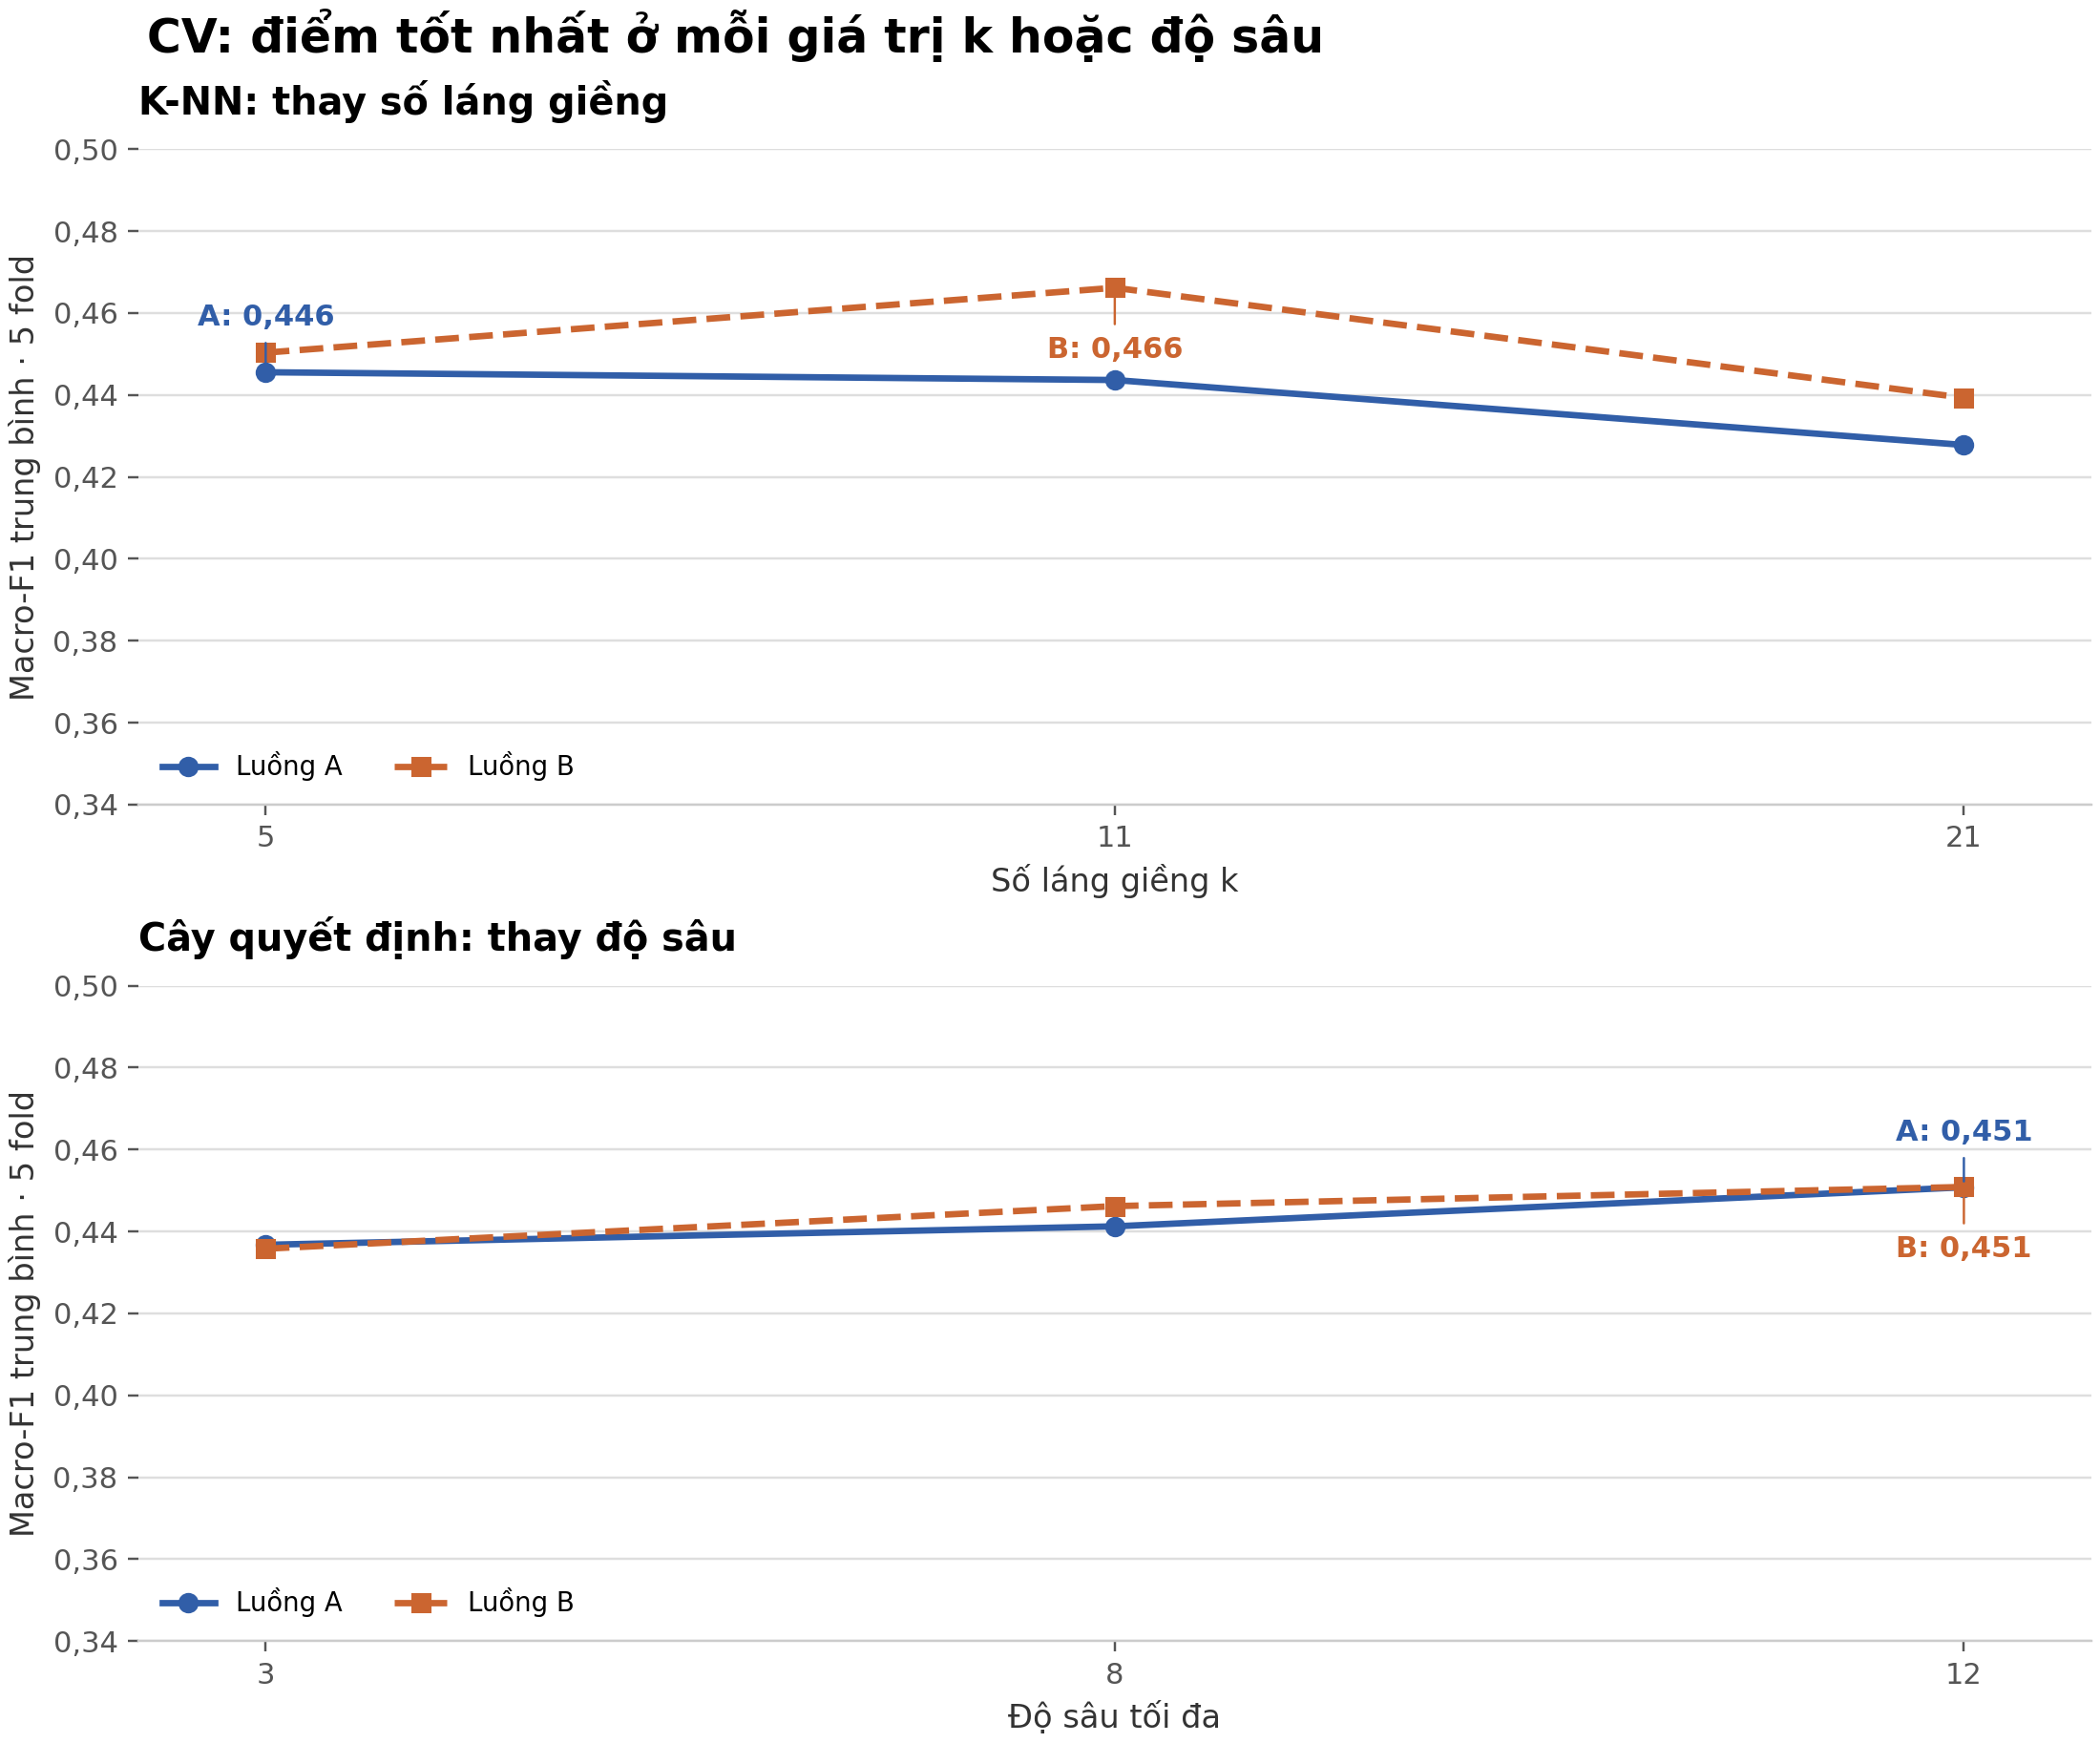
\includegraphics[width=\textwidth]{images/results/cv_curves.png}
\caption{Macro-F1 CV theo từng giá trị $k$ (K-NN) và độ sâu \texttt{max\_depth} (Cây quyết định).}\label{fig:cv-curves}
\end{figure}

Từ Hình~\ref{fig:cv-curves} và Bảng~\ref{tab:cv}, tổ hợp \textbf{B / K-NN} đạt Macro-F1 CV cao nhất ($0{,}4661$), cao hơn Baseline K-NN mặc định ($0{,}4401$) và A / K-NN ($0{,}4455$). Cấu hình được chọn dùng khoảng cách Manhattan; kết quả này không đủ để khẳng định Manhattan luôn ổn định hơn Euclid.

\section{Kết quả mô tả trên tập test đã xem}
Bảng~\ref{tab:test-summary} tổng hợp kết quả toàn diện của các mô hình baseline và 4 tổ hợp thử nghiệm trên cùng 885 mẫu test. Test đã được xem trong các lần phát triển trước và không còn là tập đánh giá cuối cùng độc lập.

\begin{table}[H]\centering\small
\caption{So sánh tổng hợp các mô hình trên tập kiểm thử (885 mẫu)}\label{tab:test-summary}
\begin{tabular}{lrrrrr}\toprule
Mô hình / Tổ hợp & Accuracy & Precision (M) & Recall (M) & Macro-F1 & Recall Dropout\\\midrule
\emph{Baseline đa số (Zero-R)} & 0,4994 & 0,1665 & 0,3333 & 0,2221 & 0,0000\\
\emph{Baseline K-NN mặc định} & 0,4972 & 0,4179 & 0,4151 & 0,4126 & 0,4401\\
\emph{Baseline Cây mặc định} & 0,4825 & 0,4343 & 0,4358 & 0,4347 & 0,4366\\\midrule
A / K-NN (tối ưu) & 0,4904 & 0,3944 & 0,4024 & 0,3955 & 0,4613\\
A / Cây (tối ưu) & 0,5277 & 0,4451 & 0,4423 & 0,4393 & \textbf{0,4859}\\
B / K-NN (tối ưu) & \textbf{0,5548} & 0,4400 & 0,4417 & 0,4279 & 0,4754\\
B / Cây (tối ưu) & 0,4938 & \textbf{0,4622} & \textbf{0,4573} & \textbf{0,4517} & 0,3732\\
\bottomrule\end{tabular}
\par\smallskip\small Precision (M) và Recall (M) ký hiệu cho giá trị trung bình vĩ mô (macro-averaged).\normalsize
\end{table}

Bảng~\ref{tab:per-class} chi tiết hóa hiệu năng từng lớp trên tập kiểm thử.

\begin{table}[H]\centering\small
\caption{Precision, Recall và F1-score theo từng lớp trên tập test}\label{tab:per-class}
\begin{tabular}{llrrrr}\toprule
Tổ hợp & Lớp & Precision & Recall & F1-score & Số mẫu thực\\\midrule
A / K-NN & Dropout & 0,4486 & 0,4613 & 0,4549 & 284\\
 & Enrolled & 0,1515 & 0,0943 & 0,1163 & 159\\
 & Graduate & 0,5830 & 0,6516 & 0,6154 & 442\\\midrule
A / Cây & Dropout & 0,4842 & 0,4859 & 0,4851 & 284\\
 & Enrolled & 0,2424 & 0,1509 & 0,1860 & 159\\
 & Graduate & 0,6088 & 0,6900 & 0,6469 & 442\\\midrule
B / K-NN & Dropout & 0,5336 & 0,4754 & 0,5028 & 284\\
 & Enrolled & 0,1833 & 0,0692 & 0,1005 & 159\\
 & Graduate & 0,6031 & 0,7805 & 0,6805 & 442\\\midrule
B / Cây & Dropout & 0,5196 & 0,3732 & 0,4344 & 284\\
 & Enrolled & 0,2638 & 0,3899 & 0,3147 & 159\\
 & Graduate & 0,6031 & 0,6086 & 0,6059 & 442\\
\bottomrule\end{tabular}
\end{table}

\begin{figure}[H]\centering
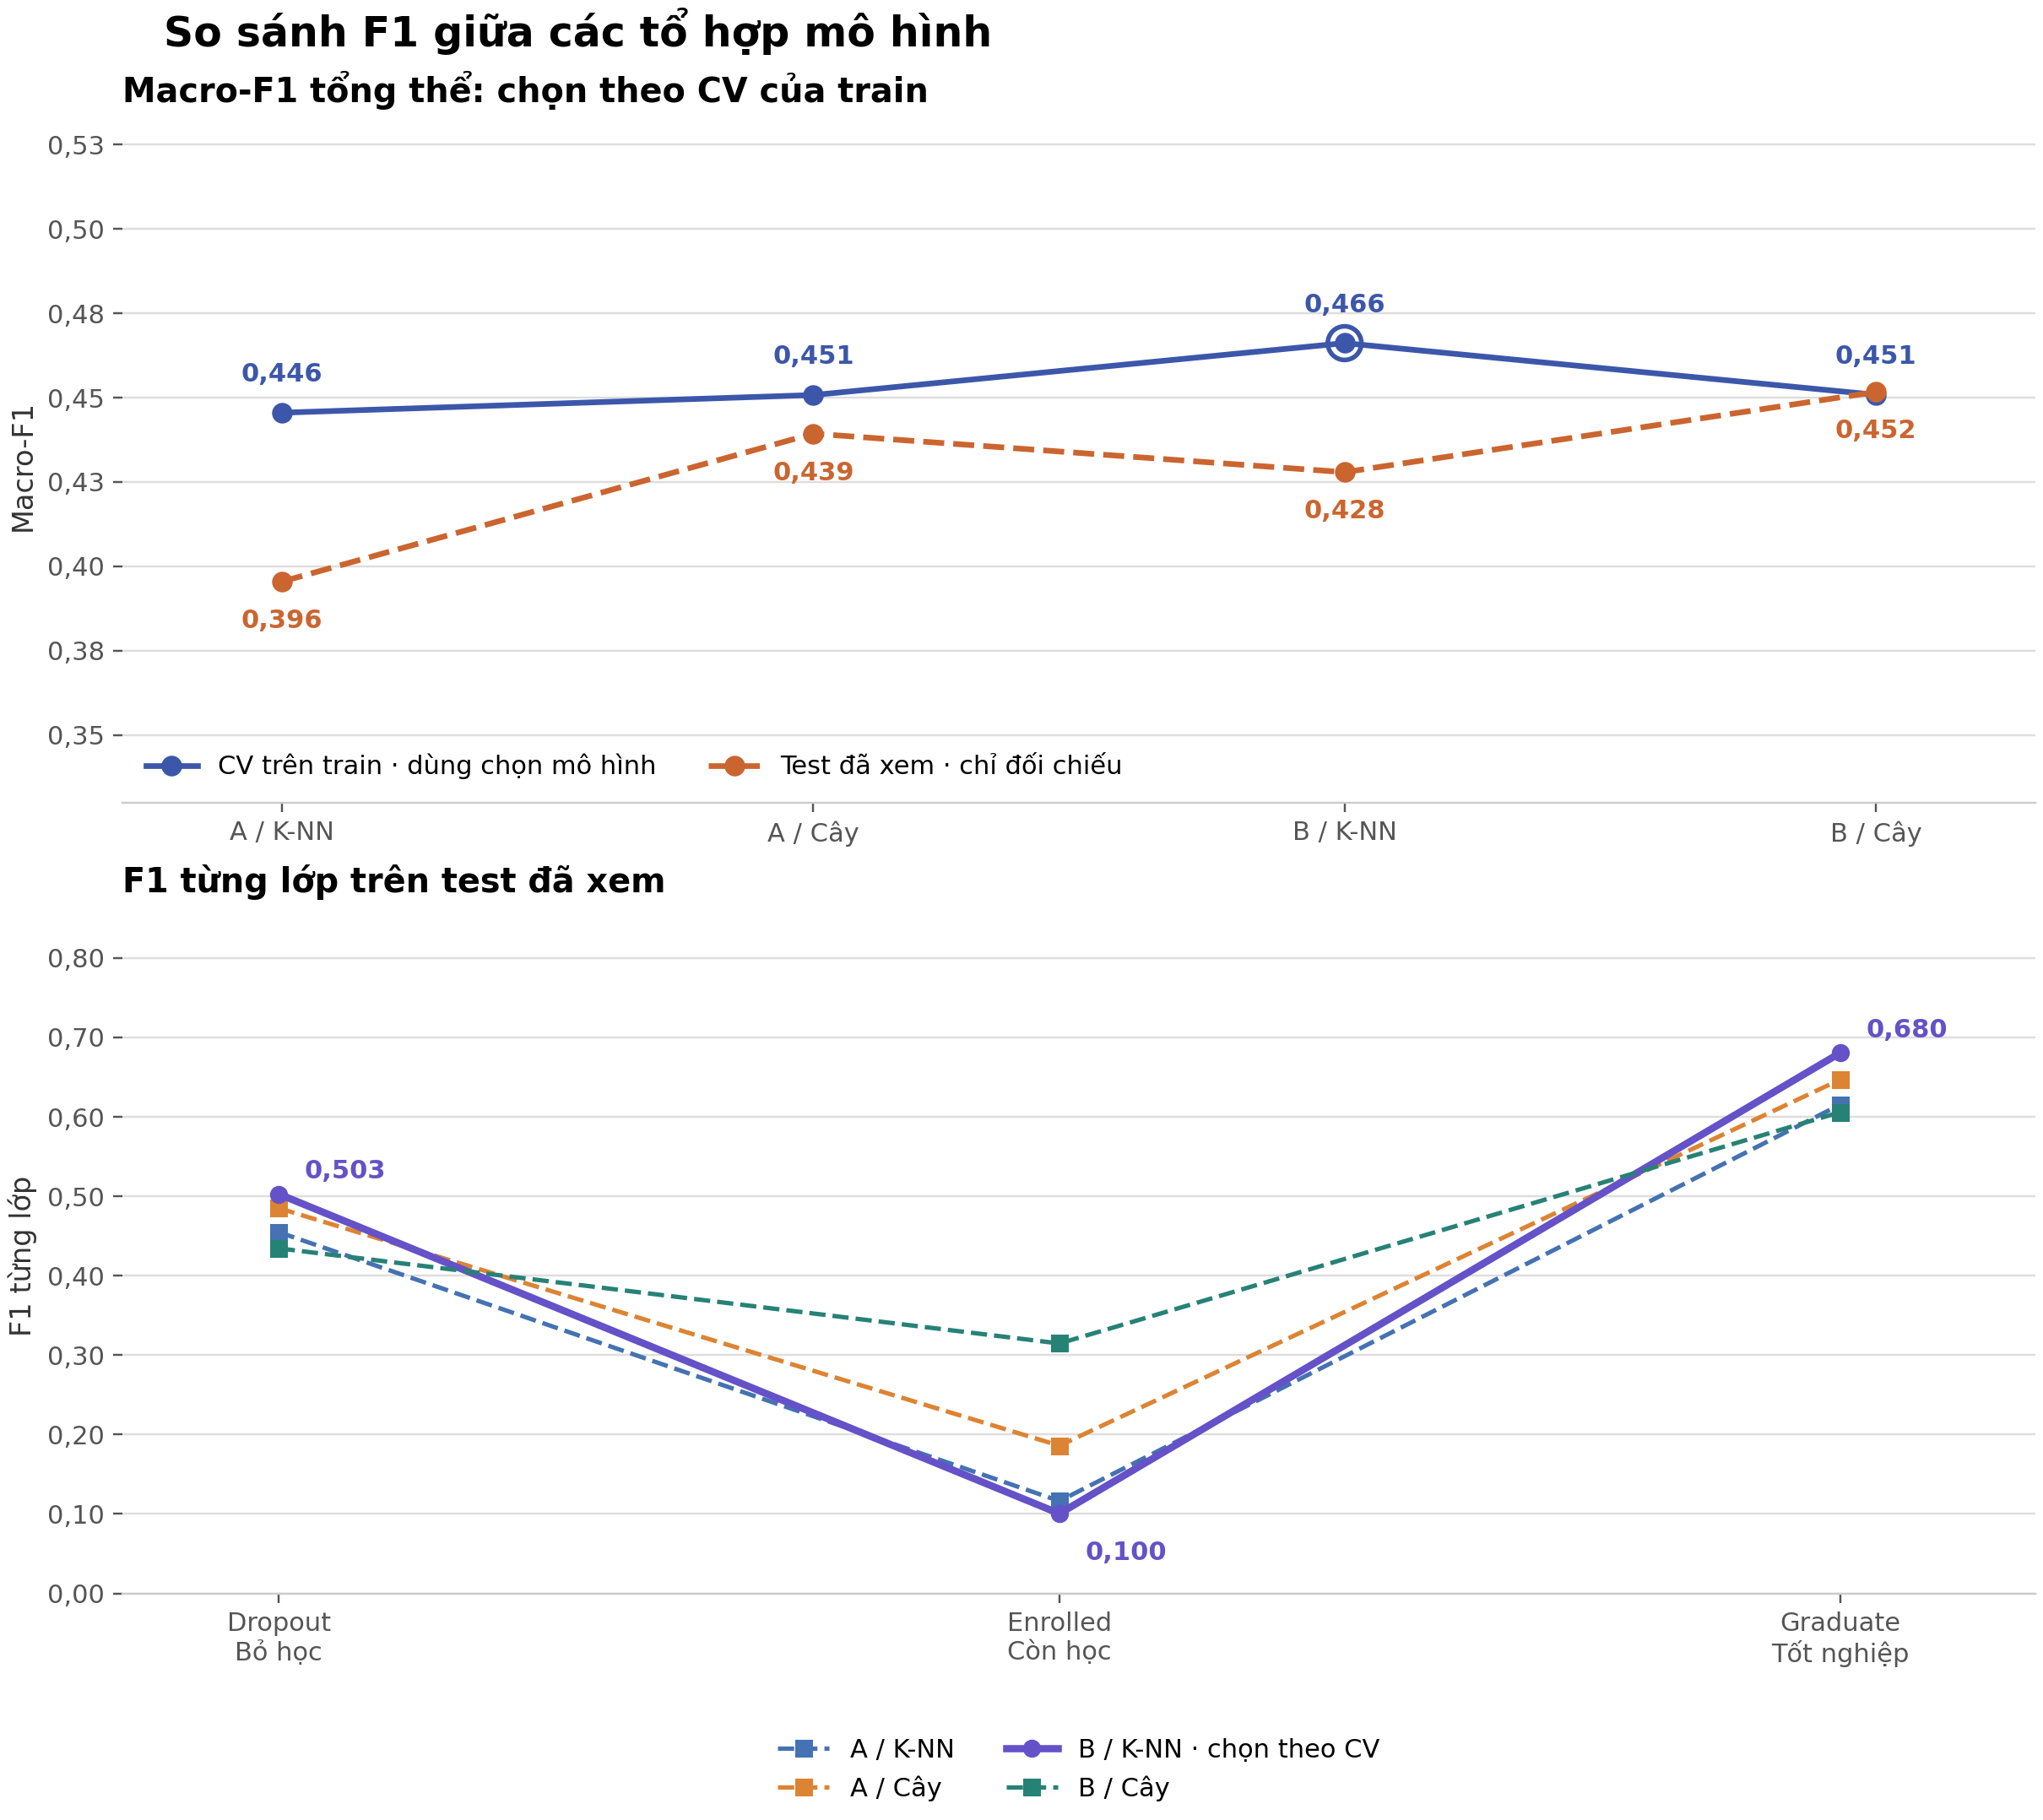
\includegraphics[width=\textwidth]{images/results/f1_algorithms.png}
\caption{So sánh Macro-F1 và F1-score từng lớp giữa các tổ hợp thử nghiệm.}\label{fig:f1-alg}
\end{figure}

\section{Phân tích Ma trận nhầm lẫn đầy đủ và kiểm tra đối chứng}\label{sec:confusion-matrices}
Hình~\ref{fig:all-cm} hiển thị ma trận nhầm lẫn trực quan của cả bốn tổ hợp thử nghiệm trên cùng 885 mẫu test (trong mỗi ô, số trên là số đếm thực tế, số dưới là tỷ lệ phần trăm theo hàng thực tế).

\begin{figure}[H]\centering
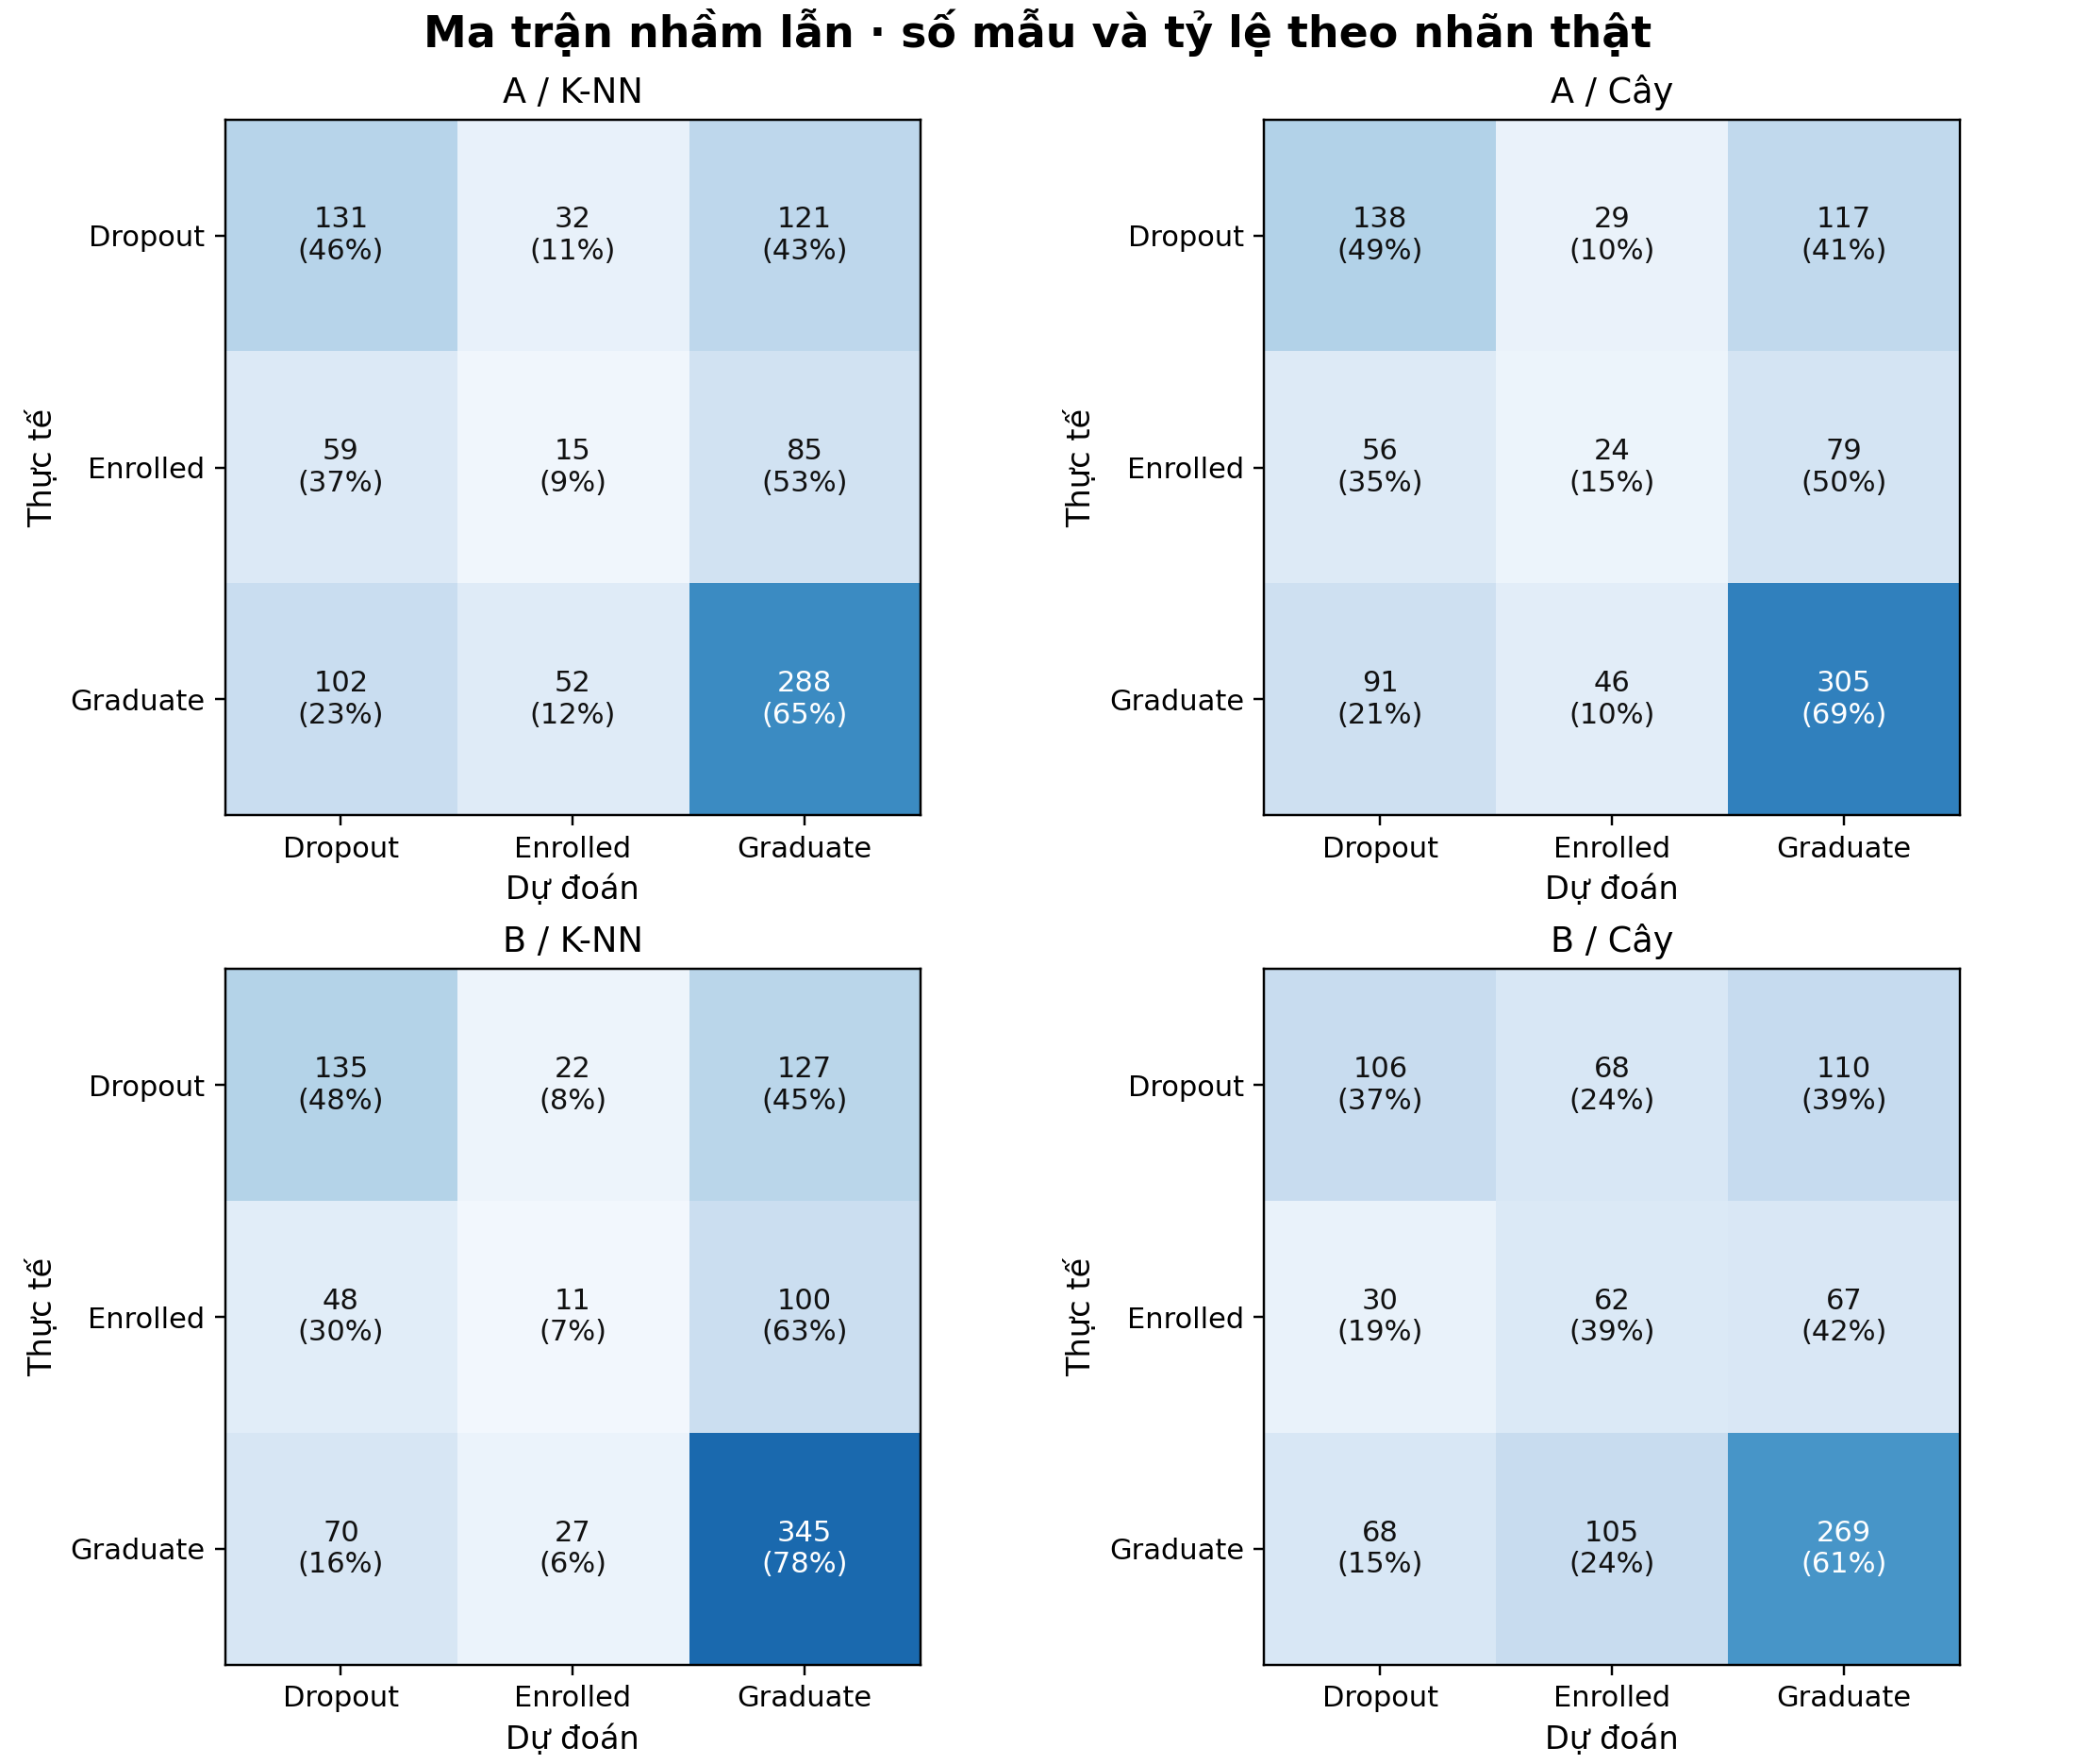
\includegraphics[width=\textwidth]{images/results/all_confusion_matrices.png}
\caption{Ma trận nhầm lẫn của 4 tổ hợp thử nghiệm trên tập test (hàng: nhãn thực, cột: dự đoán).}\label{fig:all-cm}
\end{figure}

\subsection{Làm rõ thắc mắc về Precision và Recall của lớp Dropout}
Trong quá trình đánh giá, một câu hỏi quan trọng được đặt ra: \textit{“Liệu có sự trùng hợp khi một số chỉ số của lớp Dropout xấp xỉ nhau, và điều đó phản ánh điều gì trên ma trận nhầm lẫn?”}

Dựa trên số liệu chính xác từ Bảng~\ref{tab:per-class} và Hình~\ref{fig:all-cm}:
\begin{itemize}
    \item \textbf{B / K-NN phiên bản trước}: Ma trận lưu trong \texttt{data/previous\_experiment/} có 126 Dropout đúng trong 284 Dropout thực tế; tổng số dự đoán Dropout cũng là $126+60+98=284$. Do đó precision và recall cùng bằng $126/284=0{,}4437$. Tổng 284 là số dự đoán Dropout, không phải số dự đoán đúng.
    \item \textbf{Ở mô hình B / K-NN hiện tại}: Mô hình dự đoán đúng 135 mẫu Dropout thực tế (True Positive = 135). Tổng số lần mô hình dự đoán nhãn là Dropout là $135 + 48 + 70 = 253$ mẫu. Do đó:
    \[
      \text{Precision}_{\text{Dropout}} = \frac{135}{253} = 53{,}36\%, \quad \text{Recall}_{\text{Dropout}} = \frac{135}{284} = 47{,}54\%.
    \]
    Hai giá trị này hoàn toàn khác biệt; không có hiện tượng trùng hợp số liệu ở B / K-NN.
    \item \textbf{Ở mô hình A / Cây}: True Positive Dropout là 138 mẫu. Tổng số lần mô hình gán nhãn Dropout là $138 + 56 + 91 = 285$ mẫu. Tổng số mẫu Dropout thực tế là 284 mẫu. Do đó:
    \[
      \text{Precision}_{\text{Dropout}} = \frac{138}{285} = 48{,}42\%, \quad \text{Recall}_{\text{Dropout}} = \frac{138}{284} = 48{,}59\%.
    \]
    Ở đây, Precision và Recall xấp xỉ bằng nhau chỉ đơn thuần vì tổng số mẫu dự đoán nhãn Dropout (285 mẫu) gần bằng với tổng số mẫu Dropout thực tế trong tập test (284 mẫu), chứ không phải do mô hình dự đoán đúng toàn bộ 284 mẫu. Ma trận nhầm lẫn cho thấy rõ ràng mô hình vẫn bỏ sót $29 + 117 = 146$ sinh viên Dropout thực tế sang các nhãn Enrolled và Graduate.
\end{itemize}

\subsection{Phân tích dòng chuyển dịch lỗi giữa các lớp}
Ma trận nhầm lẫn bộc lộ hai quy luật dự đoán quan trọng:
\begin{enumerate}
    \item \textbf{Khó khăn cố hữu của lớp Enrolled}: Cả A / K-NN và B / K-NN đều gặp khó khăn rất lớn trong việc nhận diện sinh viên đang theo học (Enrolled). Ở B / K-NN, chỉ có 11/159 sinh viên Enrolled được phát hiện đúng (Recall 6,92\%); có tới 100/159 sinh viên Enrolled bị mô hình dự đoán nhầm thành Graduate và 48 sinh viên bị nhầm thành Dropout.
    \item \textbf{Khác biệt của hai cấu hình cây}: Khi Cây quyết định được áp dụng trọng số lớp nghịch đảo tần suất trong Luồng B, số lượng Enrolled được nhận diện chính xác tăng vọt từ 24 mẫu (ở A / Cây) lên 62 mẫu (ở B / Cây), kéo Recall của Enrolled từ $15{,}09\%$ lên $38{,}99\%$. Hai cấu hình đồng thời khác cả tiền xử lý, trọng số lớp và tham số; không thể quy mức thay đổi này riêng cho trọng số lớp.
\end{enumerate}

\section{So sánh Luồng A và Luồng B: Tác động của tiền xử lý}
Câu hỏi cốt lõi của bài toán dữ liệu bảng là: \textit{“Thay đổi cách chuẩn bị dữ liệu có làm đổi hiệu quả mô hình không, và tại sao?”}

Kết quả thực nghiệm cho thấy rõ ràng:
\begin{itemize}
    \item \textbf{Đối với K-NN}: B/K-NN cao hơn A/K-NN 0,0206 điểm macro-F1 CV (0,4661 so với 0,4455); accuracy trên test đã xem lần lượt là 0,5548 và 0,4904. K-NN phụ thuộc vào khoảng cách; ablation trên train ở Mục~\ref{sec:ablation} kiểm tra từng thay đổi khi giữ nguyên tham số B.
    \item \textbf{Đối với Cây quyết định}: B/cây có macro-F1 test 0,4517 và nhận diện lớp Enrolled tốt hơn A/cây. Hai cấu hình đồng thời khác về tiền xử lý, trọng số lớp và tham số, vì vậy không thể quy chênh lệch riêng cho một yếu tố.
\end{itemize}


\section{Ablation trên các fold train}\label{sec:ablation}
Bảng~\ref{tab:ablation} giữ nguyên siêu tham số của từng mô hình B đã chọn và cùng năm fold, rồi bỏ một nhóm biến đổi mỗi lần. Điểm là macro-F1 trung bình trên train; không huấn luyện lại hay lựa chọn theo test. Các so sánh được thực hiện sau khi thiết kế B, là phân tích khám phá trên cùng dữ liệu và không tách biệt mọi tương tác giữa các biến.
\begin{table}[H]\centering\small
\caption{Ablation luồng B: macro-F1 trung bình trên 5 fold train}\label{tab:ablation}
\begin{tabular}{lrr}\toprule
Biến thể & B / K-NN & B / Cây\\\midrule
B đầy đủ & 0,4661 & 0,4508\\
Không gộp mã hiếm & 0,4585 & 0,4369\\
Không thêm nhóm tuổi & 0,4480 & 0,4493\\
Không thêm hiệu hai điểm & 0,4655 & 0,4471\\
Không thêm cả hai đặc trưng & 0,4529 & 0,4481\\\bottomrule
\end{tabular}\end{table}
Với K-NN đang xét, bỏ nhóm tuổi làm điểm CV giảm 0,0182; bỏ gộp mã hiếm giảm 0,0076; bỏ hiệu hai điểm giảm 0,0007. Với cây, các chênh lệch tương ứng là 0,0016; 0,0140 và 0,0037. Các con số mô tả tác động khi giữ nguyên cấu hình, không chứng minh nguyên nhân hay bảo đảm lặp lại trên dữ liệu khác. Mã và kết quả từng fold được lưu ở \texttt{scripts/evidence\_analysis.py} và \texttt{data/experiment/ablation\_cv.csv}.

\section{Khoảng biến thiên mô tả trên test đã xem}
Nhóm lấy mẫu bootstrap phân tầng 2.000 lần từ các dự đoán cố định, giữ nguyên số mẫu từng lớp; khoảng percentile 95\% của macro-F1 là [0,3649; 0,4262] cho A/K-NN, [0,4059; 0,4704] cho A/cây, [0,3981; 0,4576] cho B/K-NN và [0,4174; 0,4830] cho B/cây. So sánh cặp B/K-NN trừ A/K-NN cho chênh lệch 0,0324 với khoảng [0,0052; 0,0592]. Đây là độ biến thiên lấy mẫu có điều kiện trên test đã xem và các mô hình đã fit; không tính bất định của huấn luyện, chọn cấu hình hay độ lệch do đã xem test, nên không thay thế đánh giá trên dữ liệu độc lập mới.


\section{ROC-AUC cho cấu hình B/K-NN}
Nhóm tính ROC-AUC one-vs-rest theo từng lớp từ điểm đầu ra của B/K-NN. Trên các dự đoán out-of-fold của train, ROC-AUC macro là 0,6640; trên test đã xem, macro là 0,6433, gồm Dropout 0,6841, Enrolled 0,5774 và Graduate 0,6685. Cấu hình đã được chọn bằng CV trên cùng train trước phép tính out-of-fold nên các điểm train là mô tả sau lựa chọn; test cũng không còn độc lập với quá trình phát triển. ROC-AUC đánh giá thứ tự điểm theo từng lớp trên nhiều ngưỡng, không chứng minh các điểm đã được hiệu chỉnh xác suất. Kết quả và cách tính nằm trong \texttt{data/experiment/B\_knn\_roc\_auc.csv} và \texttt{scripts/roc\_analysis.py}.
